\documentclass[12 pt]{exam}
\usepackage{graphicx, enumitem, amsmath, amssymb}
\graphicspath{ {./images/} }
\usepackage{tikz, pgfplots}
\pgfplotsset{compat=1.16}
\usetikzlibrary{shapes,arrows}
%\usepackage{Minion Pro}
\printanswers

\title{4.1: Monopoly - Practice Problems (Answers)}
\author{Ryan Safner}
\date{ECON 306 - Fall 2019}

\begin{document}

\maketitle

Bob's Bats produces baseball bats, and has the following costs:

\begin{align*}
C(q)&=5q^2+720\\
MC(q)&=10q\\	
\end{align*}

and faces a market demand for bats:

$$q = 120-0.4p$$

where quantity is measured in thousands of bats

\begin{questions}

\question Write Bob's Marginal Revenue function.

\begin{solution}

If we can find the inverse demand (of the form $p=a+bx$, we can simply double the slope $(b)$ to get marginal revenue. We have the demand function, so solve it for $p$ to get the inverse:

\begin{align*}
q &= 120-0.4p\\
q+0.4p&=120\\
0.4p&=120-q\\
p&=300-2.5q\\
\end{align*}

This is the inverse demand function, so marginal revenue is 

$$MR(q)=300-5q$$

\end{solution}

\question Find the profit-maximizing quantity and price.

\begin{solution}

First, the quantity, we follow Rule \#1 as always: the profit maximizing $q^*$ is where $MR(q)=MC(q)$

\begin{align*}
	MR(q)&= MC(q)\\
	300-5q^=10q\\
	300&=15q\\
	20&=q^2\\
\end{align*}

Now that we know the profit-maximizing quantity, we need to find the maximum price consumers are willing to pay for 20 units. Plug this into the inverse demand function:

\begin{align*}
p&=300-2.5q\\
p&=300-2.5(20)\\
p&=300-50\\
p^*&=250\\
\end{align*}

\end{solution}

\question How much total profit does Bob's Bats earn? Should Bob stay or exit this industry in the long run?

\begin{solution}

Total profit again can be found with Rule \#2: $\pi=[p-AC(q)]q$

We first need to find the Average Cost function from total cost, by dividing it by $q$:

$$AC(q) = \frac{C(q)}{q} = \frac{5q^2+720}{q} = 5q+\frac{720}{q}$$

Now we specifically need to find the average cost at 20 units:

\begin{align*}
AC(q)&=5q+\frac{720}{q}\\
AC(20)&=5(20)+\frac{720}{20}\\
AC(20)&=100+36\\
AC(20)&=136\\
\end{align*}

Now just plug in the price, average cost, and quantity:

\begin{align*}
\pi&=[p-AC(q)]q\\
\pi&=[250-136]20\\
\pi&=[114]20\\
\pi&=2,280\\
\end{align*}

\end{solution}

\question At what price would Bob's Bats break even?

\begin{solution}

From before, we know that a firm's break even price is at the minimum of its Average Cost curve, where Average Cost is equal to Marginal Cost. First let's find the quantity where that happens:

\begin{align*}
AC(q)&=MC(q)\\
5q+\frac{720}{q}&=10q\\
\frac{720}{q}&=5q\\
720&=5q^2\\
144&q^2\\
12&=q\\
\end{align*}

This the *quantity* where AC is minimized and equal to MC. We need to find the *price*, so plug this quantity into either AC or MC. MC is easier here:

\begin{align*}
MC(q)&=10q\\
MC(12)&=10(12)\\
MC(12)&=120\\
\end{align*}

The firm breaks even at a price of \$120.
\end{solution}
	
\question How much of Bob's price is markup (over marginal cost)?

\begin{solution}

Use the Lerner Index: $L=\frac{p-MC(q)}{p}$. This will tell us what proportion of the price is markup above marginal cost.

First, we do need to find the marginal cost at $q^*=20$:

\begin{align*}
MC(q)&=10q\\
MC(20)&=10(20)\\
MC(20)&=200\\
\end{align*}

Now plug this and $p^*$ into the Lerner index:

\begin{align*}
L &= \frac{p-MC(q)}{p}\\
L &= \frac{250-200}{250}\\
L &=\frac{50}{250}\\
L &= 0.20\\
\end{align*}

The Lerner index says that 20\% of the firm's price (\$250) is markup above marginal cost (\$200).

\end{solution}

\question Calculate the price elasticity of demand at Bob's profit-maximizing price.

\begin{solution}

While you could calculate this manually, it's a lot faster to use the full Lerner Index equation: $L=\frac{p-MC(q)}{p}=-\frac{1}{\epsilon}$. Since we know $L$, we can set it equal to $-\frac{1}{\epsilon}$ and solve for $\epsilon$:

\begin{align*}
L&=-\frac{1}{\epsilon}\\
0.20&=-\frac{1}{\epsilon}\\
0.20\epsilon &=-1\\
\epsilon &=-\frac{1}{0.20}\\
\epsilon&=-5\\
\end{align*}

Demand is elastic. For every 1\% the price increases (decreases), consumers will buy 5\% less (more).
\end{solution}

\end{questions}

\begin{center} 
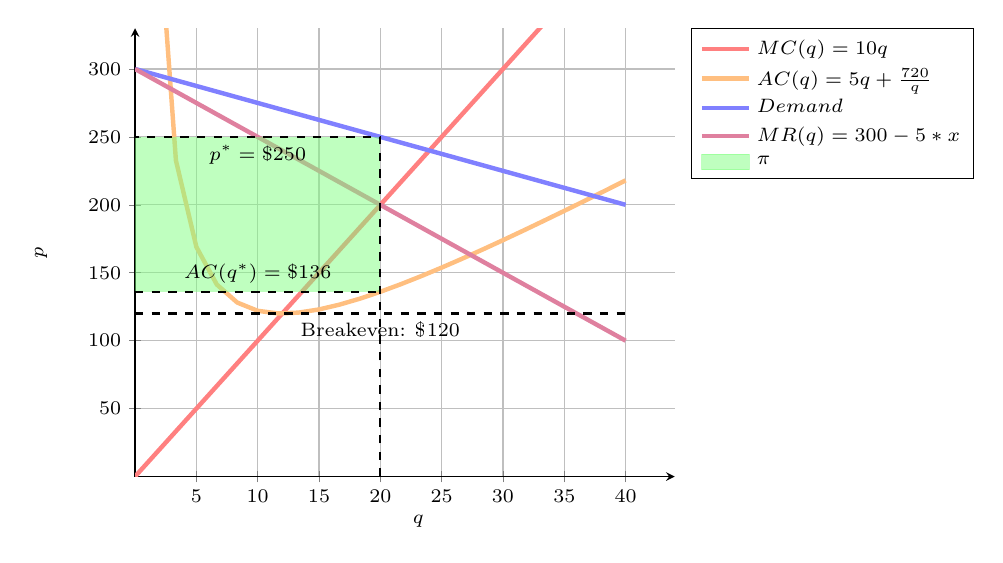
\begin{tikzpicture}\scriptsize 
	\begin{axis}[
		xlabel=$q$,
		ylabel=$p$,
		grid=major,
		legend pos=outer north east,
		legend cell align=left,
		axis lines=center,
		xtick={0,5,10,...,40},
		ytick={0,50,100,...,300},
		xmax=40,
		ymax=300,
		legend cell align=left,
		enlarge x limits={rel=0.1, upper},
		enlarge y limits={rel=0.1, upper},
		every axis y label/.style={at={(axis description cs:-0.2,0.5)},rotate=90,anchor=north},
		every axis x label/.style={at={(axis description cs:0.5,-0.1)},anchor=west},
		]
		\addplot[ultra thick, domain=0:40,red!50, samples=20]{10*x};
		\addlegendentry{$MC(q)=10q$}
		\addplot[ultra thick, domain=0:40,orange!50]{5*x+720/x};
		\addlegendentry{$AC(q)=5q+\frac{720}{q}$}
		\addplot[ultra thick, domain=0:40,blue!50]{300-2.5*x};
		\addlegendentry{$Demand$}
		\addplot[ultra thick, domain=0:40,purple!50]{300-5*x};
		\addlegendentry{$MR(q)=300-5*x$}
		\addplot[green!50, opacity=0.5, fill=green!50, draw=none, area legend] coordinates{(0,136) (0,250) (20,250) (20,136)};
		\addlegendentry{$\pi$}
		\draw[thick, dashed] (axis cs:0,120)--node[below]{Breakeven: \$120}(axis cs: 40,120);
		\draw[thick, dashed] (axis cs:20,0)--(axis cs: 20,250)--node[below]{$p^*=\$250$}(axis cs: 0,250);
		\draw[thick, dashed] (axis cs:0,136)--node[above]{$AC(q^*)=\$136$}(axis cs: 20,136);
	\end{axis}
	\end{tikzpicture}
\end{center} 

\end{document}